\chapter{MÔ HÌNH ĐỀ XUẤT}

\section{Ứng dụng các mô hình tham khảo}
Hệ thống đề xuất trong báo cáo thực tập này tích hợp ba mô hình đã được công bố, mỗi mô hình đảm nhận một vai trò cụ thể trong pipeline:
\begin{itemize}
    \item \textbf{TotalSpineSeg}~\cite{warszawer2025totalspineseg}: mô hình phân vùng và gán nhãn tự động cột sống, được dùng nguyên bản cho module phân vùng (Mục 4.2).

    \item \textbf{SpineNetV2}~\cite{windsor2022spinenetv2}: mô hình phát hiện và đánh giá bệnh lý cột sống, được dùng làm \emph{backbone} cho module grading; báo cáo tinh chỉnh mô hình này thông qua kiến trúc Hybrid (Mục~\ref{sec:phase2_arch}).

    \item \textbf{BiomedCLIP}~\cite{zhang2024biomedclip}: mô hình ngôn ngữ--thị giác y khoa pretrained trên 15M cặp ảnh--văn bản từ PubMed, được dùng làm \emph{nhánh frozen} trong kiến trúc Hybrid để cung cấp prior tổng quát (Mục~\ref{sec:phase2_arch}).
\end{itemize}
Ngoài ba mô hình trên, báo cáo cũng khảo sát và so sánh với SPINEPS~\cite{moller2024spineps}, MedCLIP-SAMv2~\cite{koleilat2025medclipsamv2} (cho phân vùng, xem Mục~\ref{sec:eval_segmentation}) và MedGemma~\cite{google2025medgemma} (cho grading, xem Mục~\ref{sec:eval_detection}) như các phương án thay thế.
Dựa trên các mô hình tham khảo đã trình bày, báo cáo thực tập này đề xuất một giải pháp hoàn chỉnh hướng tới đầy đủ các mục tiêu ở Chương 1. Luồng xử lý \emph{mục tiêu} là tuần tự: ảnh MRI $\rightarrow$ \textbf{phân vùng} (TotalSpineSeg) sinh ra mặt nạ $\rightarrow$ dùng mặt nạ để định vị vùng quan tâm (ROI) làm \textbf{đầu vào} cho mô-đun \textbf{đánh giá bệnh lý} $\rightarrow$ trình bày kết quả qua một \textbf{phần mềm giao diện} cho bác sĩ. Hình~\ref{fig:pipeline_2stage} minh họa kiến trúc tổng thể; trong đó phần nét liền là những thành phần đã thực hiện trong giai đoạn thực tập (TT2), còn phần nét đứt (màu xám) là kế hoạch hoàn thiện trong giai đoạn Đồ án tốt nghiệp (ĐATN, xem Chương 6).

\begin{figure}[H]
    \centering
    \resizebox{\textwidth}{!}{%
    \begin{tikzpicture}[
        box/.style={rectangle, draw=blue, fill=blue!8, rounded corners, minimum width=2.3cm, minimum height=1.1cm, align=center, thick, font=\small},
        outbox/.style={rectangle, draw=green!50!black, fill=green!10, rounded corners, minimum width=2.3cm, minimum height=1.1cm, align=center, thick, font=\small},
        planbox/.style={rectangle, draw=gray, dashed, fill=gray!8, rounded corners, minimum width=2.6cm, minimum height=1.1cm, align=center, thick, font=\small},
        arrow/.style={->, thick, blue!70!black},
        planarrow/.style={->, thick, gray, dashed}
    ]
        \node[box]    (input)  at (0,0)     {Ảnh MRI \\ (DICOM)};
        \node[box]    (seg)    at (4.0,0)   {\textbf{Phân vùng} \\ TotalSpineSeg};
        \node[outbox] (mask)   at (8.0,0)   {Mặt nạ \\ \scriptsize (NIfTI)};
        \node[box]    (grade)  at (12.0,0)  {\textbf{Đánh giá} \\ Hybrid grading};
        \node[outbox] (labels) at (16.0,0)  {Nhãn bệnh lý \\ \scriptsize (JSON/CSV)};
        \node[planbox](sw)      at (20.4,0)  {\textbf{Phần mềm} \\ overlay + tương tác};

        \draw[arrow] (input) -- (seg);
        \draw[arrow] (seg) -- (mask);
        \draw[planarrow] (mask) -- node[above,font=\scriptsize,text=gray]{ROI} (grade);
        \draw[arrow] (grade) -- (labels);
        \draw[planarrow] (labels) -- (sw);
        \draw[arrow] (input) to[bend right=28] node[below,font=\scriptsize]{TT2: ảnh MRI trực tiếp} (grade);
    \end{tikzpicture}}
    \caption{Kiến trúc tổng thể của giải pháp đề xuất.}
    \label{fig:pipeline_2stage}
\end{figure}


\textbf{Phân vùng cấu trúc giải phẫu với TotalSpineSeg.}
Đầu vào của hệ thống là một ảnh MRI cột sống. Ảnh này được đưa vào mô hình TotalSpineSeg. Mô hình sẽ thực hiện việc phân vùng và gán nhãn tự động. Kết quả là một tập hợp các mặt nạ phân vùng chi tiết cho từng đốt sống và đĩa đệm, cùng với một phiên bản ảnh 2D đã được tô màu để phục vụ cho việc trực quan hóa.\\

\textbf{Đánh giá các dấu hiệu bất thường với mô-đun grading tinh chỉnh.}
Ảnh MRI gốc cũng được đưa vào mô-đun grading. Mô-đun này dựa trên SpineNetV2 đã được tinh chỉnh với kiến trúc Hybrid CBAM + BiomedCLIP (chi tiết ở Mục~\ref{sec:phase2_arch}). Quy trình gồm: sử dụng kỹ thuật Hồi quy trường vector (VFR) để phát hiện các đốt sống, trích xuất các khối ảnh quanh đĩa đệm (IVVs), và đưa qua mô hình grading Hybrid để dự đoán nhãn bệnh lý. Kết quả là một file dữ liệu (JSON / CSV) chứa các điểm số định lượng, đánh giá mức độ các loại bệnh lý thoái hóa cho từng đĩa đệm.\\

\textbf{Hiện trạng và phạm vi của giai đoạn thực tập.}
Trong giai đoạn thực tập (TT2 -- bước tiền đề của ĐATN), hai mô-đun phân vùng và đánh giá bệnh lý được thực hiện \emph{độc lập}: mô-đun grading tự phát hiện đốt sống (VFR) trên ảnh MRI gốc chứ \emph{chưa tái sử dụng mặt nạ} từ TotalSpineSeg làm đầu vào. Hiện tại hai output phục vụ hai mục đích bổ trợ nhau: (i) mặt nạ phân vùng hỗ trợ trực quan hóa và cho phép bác sĩ tương tác trên ảnh; (ii) nhãn bệnh lý giúp bác sĩ biết vùng nào có dấu hiệu bất thường để kiểm tra lại. Ở giai đoạn ĐATN, mặt nạ phân vùng sẽ được \emph{dùng làm đầu vào định vị ROI} cho mô-đun grading, biến hai mô-đun rời rạc thành một pipeline tuần tự hoàn chỉnh kèm phần mềm giao diện -- để đạt đầy đủ mục tiêu đã nêu ở Chương 1 (kế hoạch chi tiết ở Chương 6). Báo cáo này tập trung vào đóng góp tinh chỉnh mô-đun grading (Mục~\ref{sec:phase2_arch}).\\

% \textbf{Lưu ý về MedGemma:} Trong quá trình khảo sát, báo cáo cũng đánh giá khả năng dùng một mô hình Vision-Language lớn (MedGemma) như một giải pháp thay thế cho mô-đun grading hoặc cho việc sinh báo cáo chẩn đoán bằng ngôn ngữ tự nhiên. Tuy nhiên, kết quả thực nghiệm trong Chương 5 cho thấy MedGemma có Recall rất thấp (6--21\%) trên các bệnh lý cột sống thắt lưng do chưa được chuyên biệt hóa, nên \emph{không được đưa vào pipeline đề xuất}. Việc fine-tune MedGemma cho bài toán này được đặt làm hướng phát triển trong Chương 6.\\

\section{Đóng góp tinh chỉnh mô-đun grading}
\label{sec:phase2_arch}

Phần này trình bày đóng góp kĩ thuật chính của báo cáo, tinh chỉnh sâu mô-đun grading được chọn từ Thí nghiệm 1. Cách tiếp cận gồm ba việc: (i) đề xuất kiến trúc \textbf{Hybrid hai nhánh} (CBAM-3D ResNet-34 trainable + BiomedCLIP frozen, hợp nhất qua Fusion MLP) để khắc phục điểm yếu Severe Recall thấp của SpineNetV2 baseline, (ii) triển khai pipeline xử lý mất cân bằng (Focal Loss + Uncertainty Loss + minority oversampling), và (iii) kiểm chứng tổng quát hóa qua transfer learning sang SPIDER 8-label (Mục~\ref{sec:phase2_eval}).

\subsection{Tổng quan kiến trúc Hybrid}
Báo cáo đề xuất một kiến trúc \textbf{Hybrid hai nhánh} (Hình~\ref{fig:hybrid_arch}) gồm: một nhánh CBAM-3D ResNet-34 \emph{trainable} học đặc trưng trực tiếp từ khối ảnh 3D của đĩa đệm, một nhánh BiomedCLIP \emph{frozen} cung cấp \emph{prior}, đặc trưng nền tổng quát đã học sẵn từ pretraining trên 15 triệu cặp ảnh--văn bản y khoa. Hai nhánh được hợp nhất qua một mô-đun MLP nhỏ, sau đó dẫn vào các head phân loại đa nhiệm cho từng nhãn bệnh lý.

\begin{figure}[H]
    \centering
    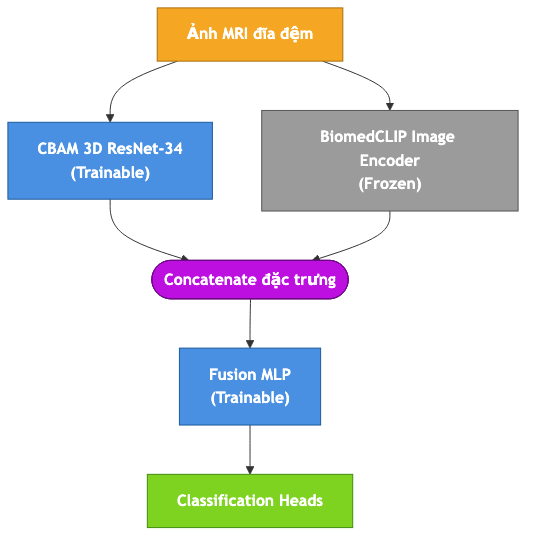
\includegraphics[width=0.5\textwidth]{cslt/hybrid_architecture.png}
    \caption{Kiến trúc Hybrid hai nhánh.}
    \label{fig:hybrid_arch}
\end{figure}

Hình~\ref{fig:training_arch} và Hình~\ref{fig:inference_arch} mô tả riêng biệt hai giai đoạn huấn luyện và suy luận. Trong giai đoạn huấn luyện, dữ liệu đi qua thêm augmentation và minority oversampling; gradient chỉ đi qua nhánh trainable (CBAM-ResNet) còn BiomedCLIP frozen hoàn toàn. Loss tổng hợp gồm Focal Loss và Uncertainty Loss được tính ở các head. Trong giai đoạn suy luận, không có augmentation và loss, chỉ thực hiện forward pass để sinh xác suất dự đoán.

\begin{figure}[H]
    \centering
    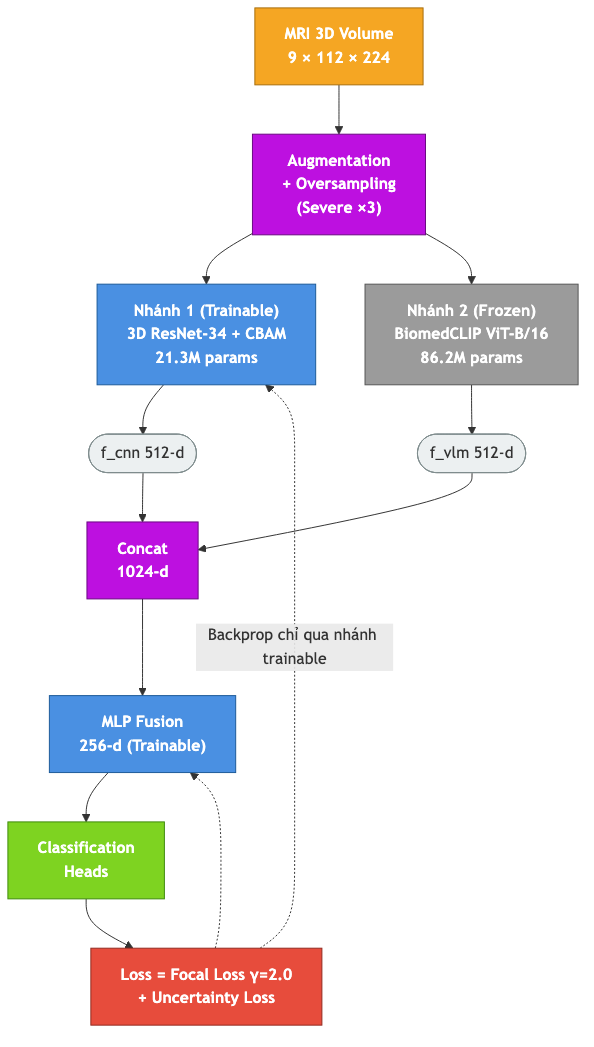
\includegraphics[width=0.58\textwidth]{cslt/training_architecture.png}
    \caption{Kiến trúc huấn luyện.}
    \label{fig:training_arch}
\end{figure}

\begin{figure}[H]
    \centering
    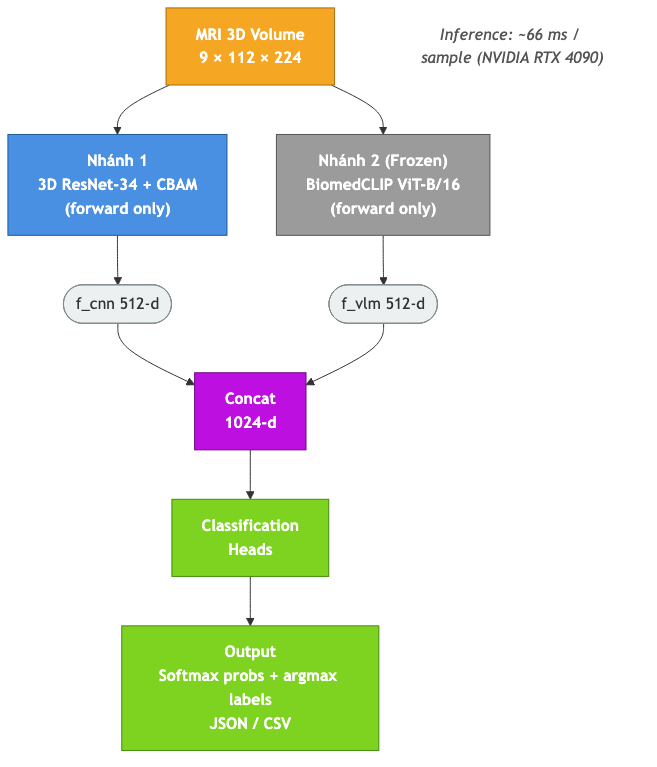
\includegraphics[width=0.6\textwidth]{cslt/inference_architecture.png}
    \caption{Kiến trúc suy luận.}
    \label{fig:inference_arch}
\end{figure}

\subsection{Chi tiết hai nhánh và mô-đun hợp nhất}

\textbf{Nhánh CBAM-3D ResNet-34:} Dựa trên 3D ResNet-34 với convolution 3D kernel $3 \times 3 \times 3$, stride chỉ áp dụng trên hai chiều không gian $(H, W)$ và giữ nguyên chiều slice $D = 9$. Backbone được khởi tạo bằng trọng số pretrained trên Med3D~\cite{chen2019med3d}. Input là khối ảnh đĩa đệm kích thước $(9, 112, 224)$. CBAM được chèn sau mỗi stage của ResNet (4 stages: 64, 128, 256, 512 kênh), vị trí cuối stage là nơi đặc trưng đã đủ trừu tượng để cơ chế chú ý có thể nhìn được pattern ý nghĩa (vùng đĩa đệm tổn thương vs vùng mô lành), nhưng chưa quá nén để mất hết thông tin không gian. Đầu ra sau global average pooling 3D là embedding $f_{cnn}$ 512-d.


\textbf{Nhánh BiomedCLIP:} Cung cấp \emph{prior tổng quát} từ pretraining quy mô lớn. Báo cáo chọn BiomedCLIP \cite{zhang2024biomedclip} thay vì MedCLIP hoặc PMC-CLIP vì BiomedCLIP có dataset pretraining lớn nhất (15M cặp PubMed) và đa dạng modality (MRI, CT, X-ray, mô bệnh học). 

\textbf{Fusion MLPvà heads phân loại:} Hai embedding $f_{cnn}$ và $f_{vlm}$ (mỗi cái 512-d) được ghép thành vector 1024-d, đi qua MLP hai lớp (hidden 256, ReLU, dropout 0.3) cho ra embedding chia sẻ $f_{shared}$ 256-d. Concat + MLP đơn giản hơn các cơ chế gating phức tạp nhưng đủ cho dataset quy mô vừa. 

\subsection{Pipeline xử lý mất cân bằng lớp}
Bài toán RSNA có phân bố nhãn rất mất cân bằng: trên trục Severity, Normal/Mild chiếm $\sim$78\%, Moderate $\sim$18\%, Severe chỉ $\sim$4\%. Mô hình baseline huấn luyện với Cross-Entropy thuần thường rơi vào trạng thái lười, chỉ học dự đoán Normal/Mild để đạt accuracy cao, trong khi Severe Recall gần như bằng 0. Báo cáo áp dụng ba kĩ thuật phối hợp để xử lý vấn đề này:

\textbf{(a) Focal Loss \cite{lin2017focal}.} Giảm trọng số đóng góp của các mẫu dễ (mẫu Normal/Mild đã có xác suất dự đoán $p_t$ cao) và tăng cho các mẫu khó (Severe có $p_t$ thấp). Công thức:
\begin{equation}
    FL(p_t) = -\alpha_t (1 - p_t)^\gamma \log(p_t)
\end{equation}
với $\gamma = 2.0$ là hyperparameter chuẩn. 

\textbf{(b) Uncertainty Loss \cite{kendall2018multitask}.} Học trọng số động giữa các nhãn. Mỗi nhiệm vụ có một tham số log-variance $\sigma_k$ được học cùng với weight của model. Loss tổng cho 5 nhiệm vụ:
\begin{equation}
    \mathcal{L}_{total} = \sum_{k=1}^{5} \left( \frac{1}{2 \sigma_k^2} \mathcal{L}_k + \log \sigma_k \right)
\end{equation}
Nếu một nhiệm vụ có loss cao (ví dụ subarticular stenosis khó hơn các nhãn khác), tham số $\sigma_k$ sẽ tự động tăng lên để giảm trọng số cho nhiệm vụ đó. Cơ chế này ngăn nhiệm vụ khó áp đảo và làm bias các nhiệm vụ dễ hơn.

\textbf{(c) Minority oversampling.} Với mỗi epoch, các sample chứa ít nhất một head có nhãn Severe sẽ được lặp lại 3 lần (oversample factor = 3). Cách này làm tăng đáng kể số iteration mà model thấy các mẫu Severe, từ đó cải thiện khả năng học của lớp hiếm. Hệ số oversampling được điều chỉnh thực nghiệm, giá trị quá cao (5 - 10) gây overfitting trên các mẫu Severe ít ỏi, giá trị quá thấp (1 - 2) không đủ tác động.

